\chapter{ADAPTER}

Il pattern Adapter è un design pattern \underline{strutturale} che consente a due interfacce incompatibili di lavorare insieme, nello specifico consente a una classe di 
funzionare da adattatore tra queste due interfacce, consentendo loro di collaborare senza dover modificare il loro codice sorgente.

\section{Applicabilità}

Vogliamo usare una classe esistente ma la sua interfaccia non è compatibile con l'interfaccia che ci serve oppure vogliamo creare una classe riusabile che collaborerà 
con classi scorrelate.

\section{Struttura}

Abbiamo due varianti di questo pattern, una con ereditarietà ed una con object composition e delega.

Nella prima variante abbiamo una classe, Adapter, che implementa l'interfaccia che ci serve, estendendo un'altra classe esistente, Adaptee, cosicchè i metodi 
dell'interfaccia chiameranno i metodi della superclasse Adaptee.

\begin{figure}[H]
    \centering 
    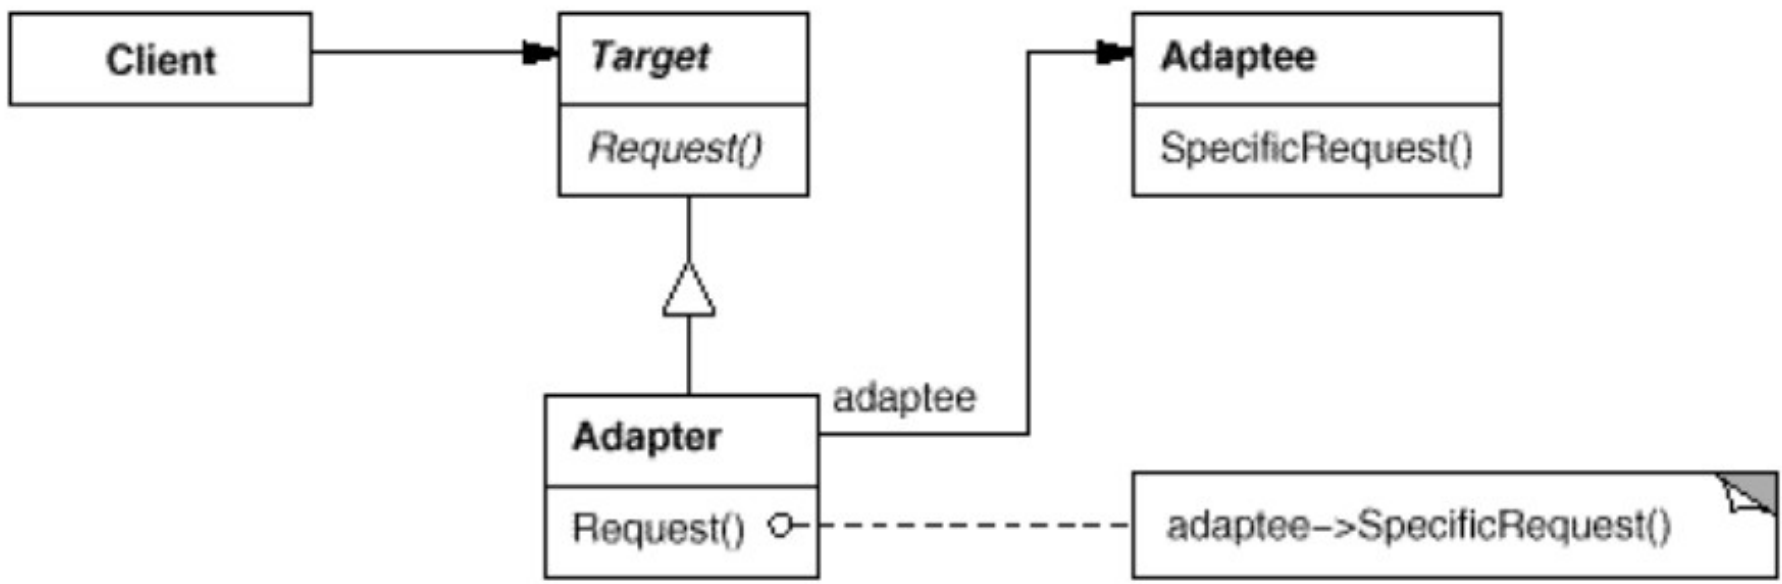
\includegraphics[width=0.5\linewidth]{adapter/struttura_adapter_composition.png}    
\end{figure}

Nella seconda variante, Adapter implementa l'interfaccia che ci serve delegando ad un Adaptee e i metodi dell'interfaccia chiamarenno dei metodi sull'oggetto Adaptee.
\begin{figure}[H]
    \centering
    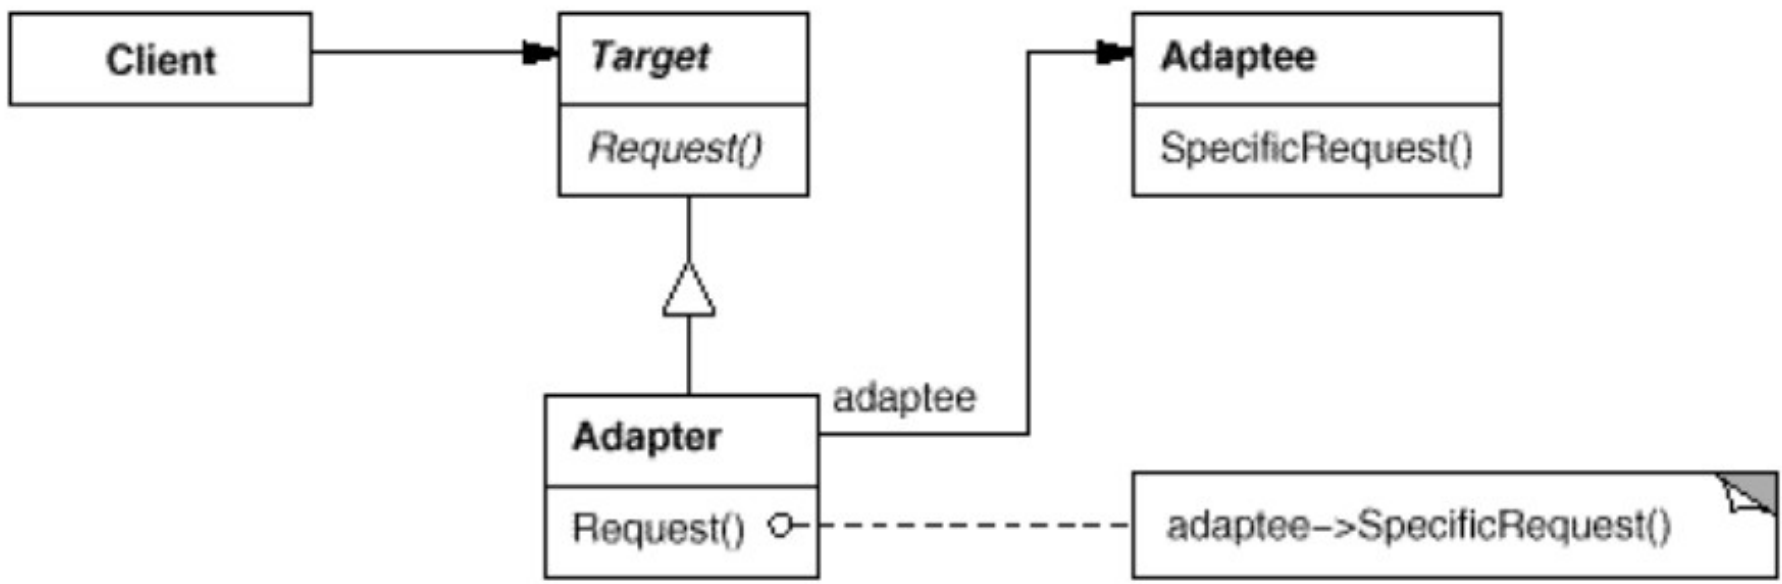
\includegraphics[width=0.5\linewidth]{adapter/struttura_adapter_composition}
\end{figure}

\textbf{Target} definisce l'interfaccia del dominio usata dai Client;

\textbf{Client} collabora con gli oggetto conformi all'interfaccia Target;

\textbf{Adaptee} l'interfaccia esistente da adattare;

\textbf{Adapter} adatta l'interfaccia Adaptee a Target.

\medskip
Il Client, a runtime, chiama operazioni su oggetto Adapter, staticamente di tipo Target, che a sua volta gestisce le operazioni chiamando in modo opportuno delle operazioni 
di Adaptee.

\section{Conseguenze}

Nella versione basata su ereditarietà
\begin{itemize}
    \item la classe Adapter adatta \underline{un certo tipo concreto} di Adaptee, quindi se volessi adattare una sottoclasse di Adaptee, allora dovremmo creare un 
    nuovo adapter;
    \item possiamo ridefinire i metodi Adaptee in quanto è superclasse di Adapter;
    \item non introduciamo un nuovo livello di indirezione perchè non c'è object composition.
\end{itemize}

Nella versione basata su object composition
\begin{itemize} 
    \item si può adattare \underline{qualsiasi} istanza di Adaptee;
    \item possiamo aggiugere del comportamento prima o dopo le operazioni di Adaptee;
    \item introduciamo un ulteriore di livello di indirezione.
\end{itemize}

\textbf{N.B.} In linguaggi tipo java, in cui ereditarietà implica subtyping, bisogna usare la versione object composition.

\section{Altro utilizzo di Adapter}

Esiste un altro caso d'uso di questo pattern.

Supponiamo di avere un'interfaccia con tanti metodi astratti che sono correlati tra loro (altrimenti si violerebbe ISP) e di avere una classe che la implementa.

Implementare un'interfaccia significa implementare tutti metodi dell'interfaccia anche se a noi iteressano determinati metodi.

Ecco che interviene l'Adapter, che fa da ponte tra l'interfaccia, dando un'implementazione di default a tutti i metodi dell'interfaccia (tipicamente vuota), e la 
nostra classe, che estende Adapter e reimplementa solo i metodi che gli servono.

\medskip
\textbf{N.B.}L'implementazione di default si applica facilmente solo ai metodi void.

\section{Adapter vs default methods}

Questo pattern è un'alternativa ai default methods in quanto invece di stabilire una volta per tutte l'implementazione di default nell'interfaccia, con l'Adapter, noi 
non la tocchiamo e lasciamo più libertà allo sviluppatore.
